%% Adapted from SoftwareX original software publication template.
%% Original template Copyright 2026 Elsevier Ltd, distributed under LPPL 1.2 or later.
%% Changes: manuscript content, fitted metadata table, figures, mathematical notation.
\documentclass[preprint,12pt,a4paper]{elsarticle}
\usepackage{amssymb,amsmath,booktabs,tabularx,listings,xcolor,placeins,array}
\usepackage[hidelinks]{hyperref}
\setlength{\parindent}{0pt}
\setlength{\parskip}{4pt}
\lstset{basicstyle=\ttfamily\footnotesize,breaklines=true,frame=single,columns=fullflexible,showstringspaces=false}
\emergencystretch=2em
\journal{SoftwareX}
\begin{document}
\begin{frontmatter}
\title{TPMS Lab: A Python package for graded solid and pore-fluid meshes with verified COMSOL workflows}
\author{[Author names to be supplied]}
\address{[Affiliations and postal addresses to be supplied]}
\begin{abstract}
TPMS Lab is a Python package for generating graded lattice solid meshes and complementary pore-fluid meshes from implicit periodic fields. Shared interface nodes and triangles provide a conforming two-phase discretization with connected-domain and boundary labels. The package includes a Python API, command-line tools, a local browser interface, mesh diagnostics and an optional COMSOL bridge. Seventy-seven automated tests and three COMSOL pore-flow demonstrations verify partitioning, import, solution storage and reopening. Earlier solid-only benchmarks quantify a local quality-selection trade-off and six elasticity workflow checks. The software supports reproducible simulation preparation without smooth CAD reconstruction; mesh convergence and deformation-coupled fluid--structure interaction remain unverified.
\end{abstract}
\begin{keyword}
TPMS \sep graded lattices \sep solid--fluid domains \sep tetrahedral meshing \sep Python \sep COMSOL
\end{keyword}
\end{frontmatter}
\clearpage
\section*{Required Metadata}
\section*{Current code version}
\begin{table}[!ht]
\small\renewcommand{\arraystretch}{1.15}
\begin{tabularx}{\textwidth}{@{}p{.04\textwidth}>{\raggedright\arraybackslash}p{.34\textwidth}>{\raggedright\arraybackslash}X@{}}
\toprule
Nr. & Code metadata description & Value \\
\midrule
C1 & Current code version & 0.3.0rc1; unpublished release candidate \\
C2 & Permanent GitHub link to code/repository used for this code version & [Public GitHub repository and immutable release link to be supplied] \\
C3 & Legal Code License & MIT; third-party notices retained \\
C4 & Code versioning system used & [Confirm repository version-control system before submission] \\
C5 & Software code languages, tools, and services used & Python; Java for the optional COMSOL bridge; JavaScript/HTML/CSS for the local interface \\
C6 & Compilation requirements, operating environments \& dependencies & Python $\geq$3.11; NumPy, SciPy, trimesh; optional Flask. Tested on Windows/Python 3.12. COMSOL 6.3 and suitable licences are external requirements for solver integration only. \\
C7 & If available Link to developer documentation/manual & [Public documentation link to be supplied]; README.md and docs accompany source \\
C8 & Support email for questions & [Maintainer email to be supplied] \\
\bottomrule
\end{tabularx}
\caption{Code metadata. Bracketed fields must be completed before submission.}
\end{table}
\FloatBarrier
\FloatBarrier
\section{Motivation and significance}

Triply periodic minimal surface (TPMS)-derived lattices are commonly described using periodic implicit fields and level-set thresholds. Grading changes the local distribution of solid and pore space. A surface representation is useful for visualization or fabrication, but volume-based simulation also requires a discretization of the relevant phases and identification of material domains and boundaries. For pore-resolved flow, the empty region in a solid-only model must become an explicit fluid domain. Retaining the correspondence between these phases is therefore part of simulation preparation.

Existing tools already address substantial parts of this problem. LattGen generates uniform, graded and hybrid TPMS-derived structures and exports STL surfaces \cite{lattgen}. TPMeSh exports surface meshes and tetrahedral volume meshes \cite{tpmesh}. LisbonTPMS-tool provides cell-size and density grading, surface export and voxel-based eight-node hexahedral finite-element meshes \cite{lisbon}. Consequently, neither grading nor volume-mesh generation alone constitutes the contribution of TPMS Lab. Guaranteed-quality implicit meshing also has a substantial history, including isosurface stuffing \cite{stuffing}.

TPMS Lab provides a reusable Python workflow linking density parameters to labelled solid and complementary pore-fluid meshes, numerical diagnostics and saved COMSOL models. The implementation avoids a prerequisite conversion to a smooth CAD solid. Its contribution is the integration of conforming complementary phase meshing, explicit connected-domain and interface metadata, and inspectable solver verification. The present evidence establishes functionality for the included cases; it does not establish superiority over existing meshers, new TPMS families or a general mesh-quality guarantee.

\FloatBarrier
\section{Software description}

\subsection{Software architecture}

Figure~\ref{fig:workflow} summarizes the workflow. The package separates field definitions and configuration, volume generation, complementary-domain assembly, export and solver integration. The public entry points are Config, generate and save\_model. A command-line interface exposes configuration generation, mesh generation and an optional browser application. NumPy, SciPy and trimesh are core dependencies. Flask is optional; COMSOL is not needed to generate or inspect mesh files. The optional Java bridge targets a separately installed, licensed COMSOL environment.

A configuration records the field family, sheet or network representation, dimensions, cell counts, phases, sampling resolution, density law and meshing strategy. A restricted expression parser supports custom fields. The reference registry adapts the attributed LattGen formulas and contains 29 labels representing 27 distinct expressions. These trigonometric fields are level-set approximations rather than exact minimal surfaces. Eight density profiles are supported. Cell counts remain fixed along each axis: spatial variation of cell size is not implemented in this release.


\begin{figure}[!htbp]
\centering
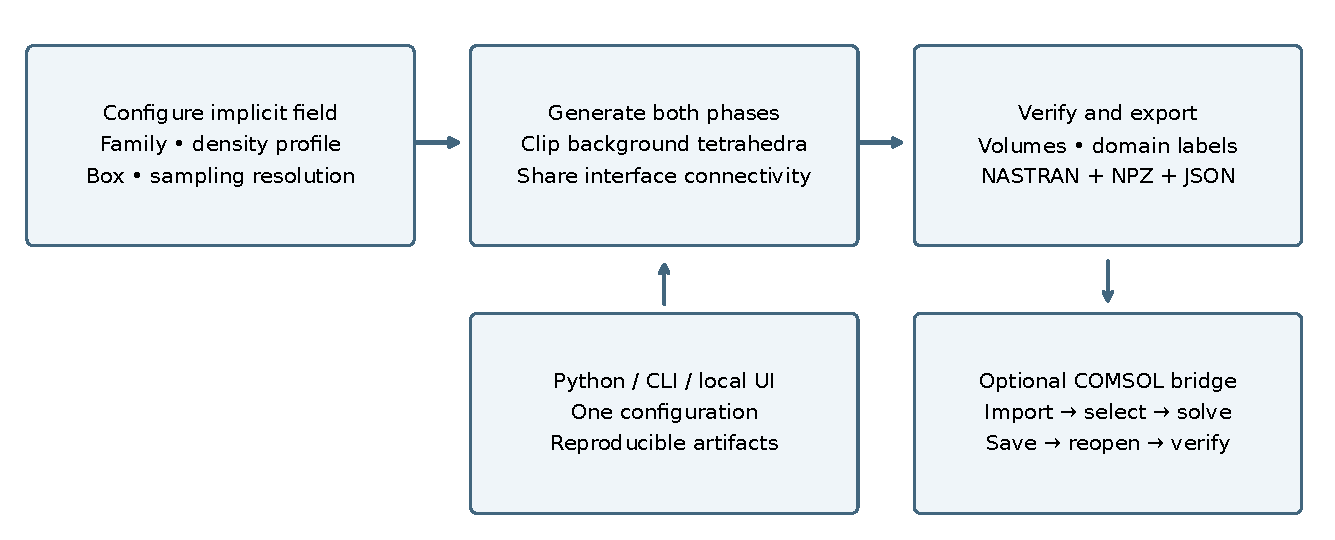
\includegraphics[width=1.0\textwidth]{fig1_workflow.pdf}
\caption{Package architecture and optional solver workflow. Geometry generation and mesh verification do not require COMSOL.}
\label{fig:workflow}
\end{figure}

\subsection{Software functionalities}

Density calibration uses the empirical cumulative distribution of a periodically sampled unit cell. At each background-grid vertex, the requested density determines a threshold q. For sheet structures, solid material satisfies $q-f\geq0$ and $q+f\geq0$, where f is the periodic field. Each Cartesian voxel is split into six tetrahedra, and the two fields are interpolated linearly within each tetrahedron. The inequalities are clipped separately; this preserves the sheet interpretation rather than interpolating an absolute-value field after sampling. Threshold variation is not equivalent to a prescribed physical wall-thickness field.

Shared cut vertices are identified by the background edge and clipping plane. Deterministic polygon triangulation provides compatible faces on adjacent cells. The baseline uses a pulling triangulation. An optional quality\_fan strategy compares this with an interior-centroid fan and accepts the candidate only when its worst tetrahedral mean-ratio quality improves and its volume agrees with the baseline. The quality measure is $Q=12(3V)^{2/3}/\sum_{i=1}^{6}l_i^2$, with six edge lengths l. This local choice preserves boundary triangles but can increase the number of elements and reduce median quality.

Figure~\ref{fig:interface} illustrates the conforming phase partition. The solid\_fluid mode additionally meshes the complement inside the same bounding box. For a sheet, the two pore regions are obtained by reversing each clipping inequality separately. Original and cut-edge identities are shared across phases; newly added interior vertices remain local to their own regions. The assembled mesh is checked for positive tetrahedral volumes, opposite orientations of shared faces, matching solid--fluid interface triangles and conservation of the bounding-box volume. An unmatched internal boundary causes rejection. Connected domains are computed using shared tetrahedral faces, allowing separate labyrinths to retain separate labels.

The return value contains points, tetrahedra, connected-domain labels and phase identifiers (1 for solid, 2 for fluid). It also includes the shared interface, separate phase boundaries and a diagnostic report. In dual-domain output, the exported boundary array includes the external boundary and the internal solid--fluid interface once. Each connected domain has a NASTRAN PSOLID property ID; solid and fluid external faces have separate property IDs, and the interface has its own boundary ID. A JSON mapping distinguishes mesh labels from solver entity numbers.

Exports include NASTRAN volume and boundary elements, compressed NumPy arrays, separate solid/fluid STL previews, configuration, diagnostics, dependency versions and file hashes. The previews contain surfaces only. COMSOL supports importing NASTRAN meshes and creating selections from property IDs \cite{comsol}. The bridge resolves those imported selections, creates named phase and interface selections, and assigns separate demonstration materials. It checks the imported connected-domain volumes and embedded tetrahedron count before and after saving the MPH file. The representation is a mesh-defined computational domain, not a smooth STEP or NURBS solid. Geometry-level Boolean operations are not a verified feature of the software.


\begin{figure}[!htbp]
\centering
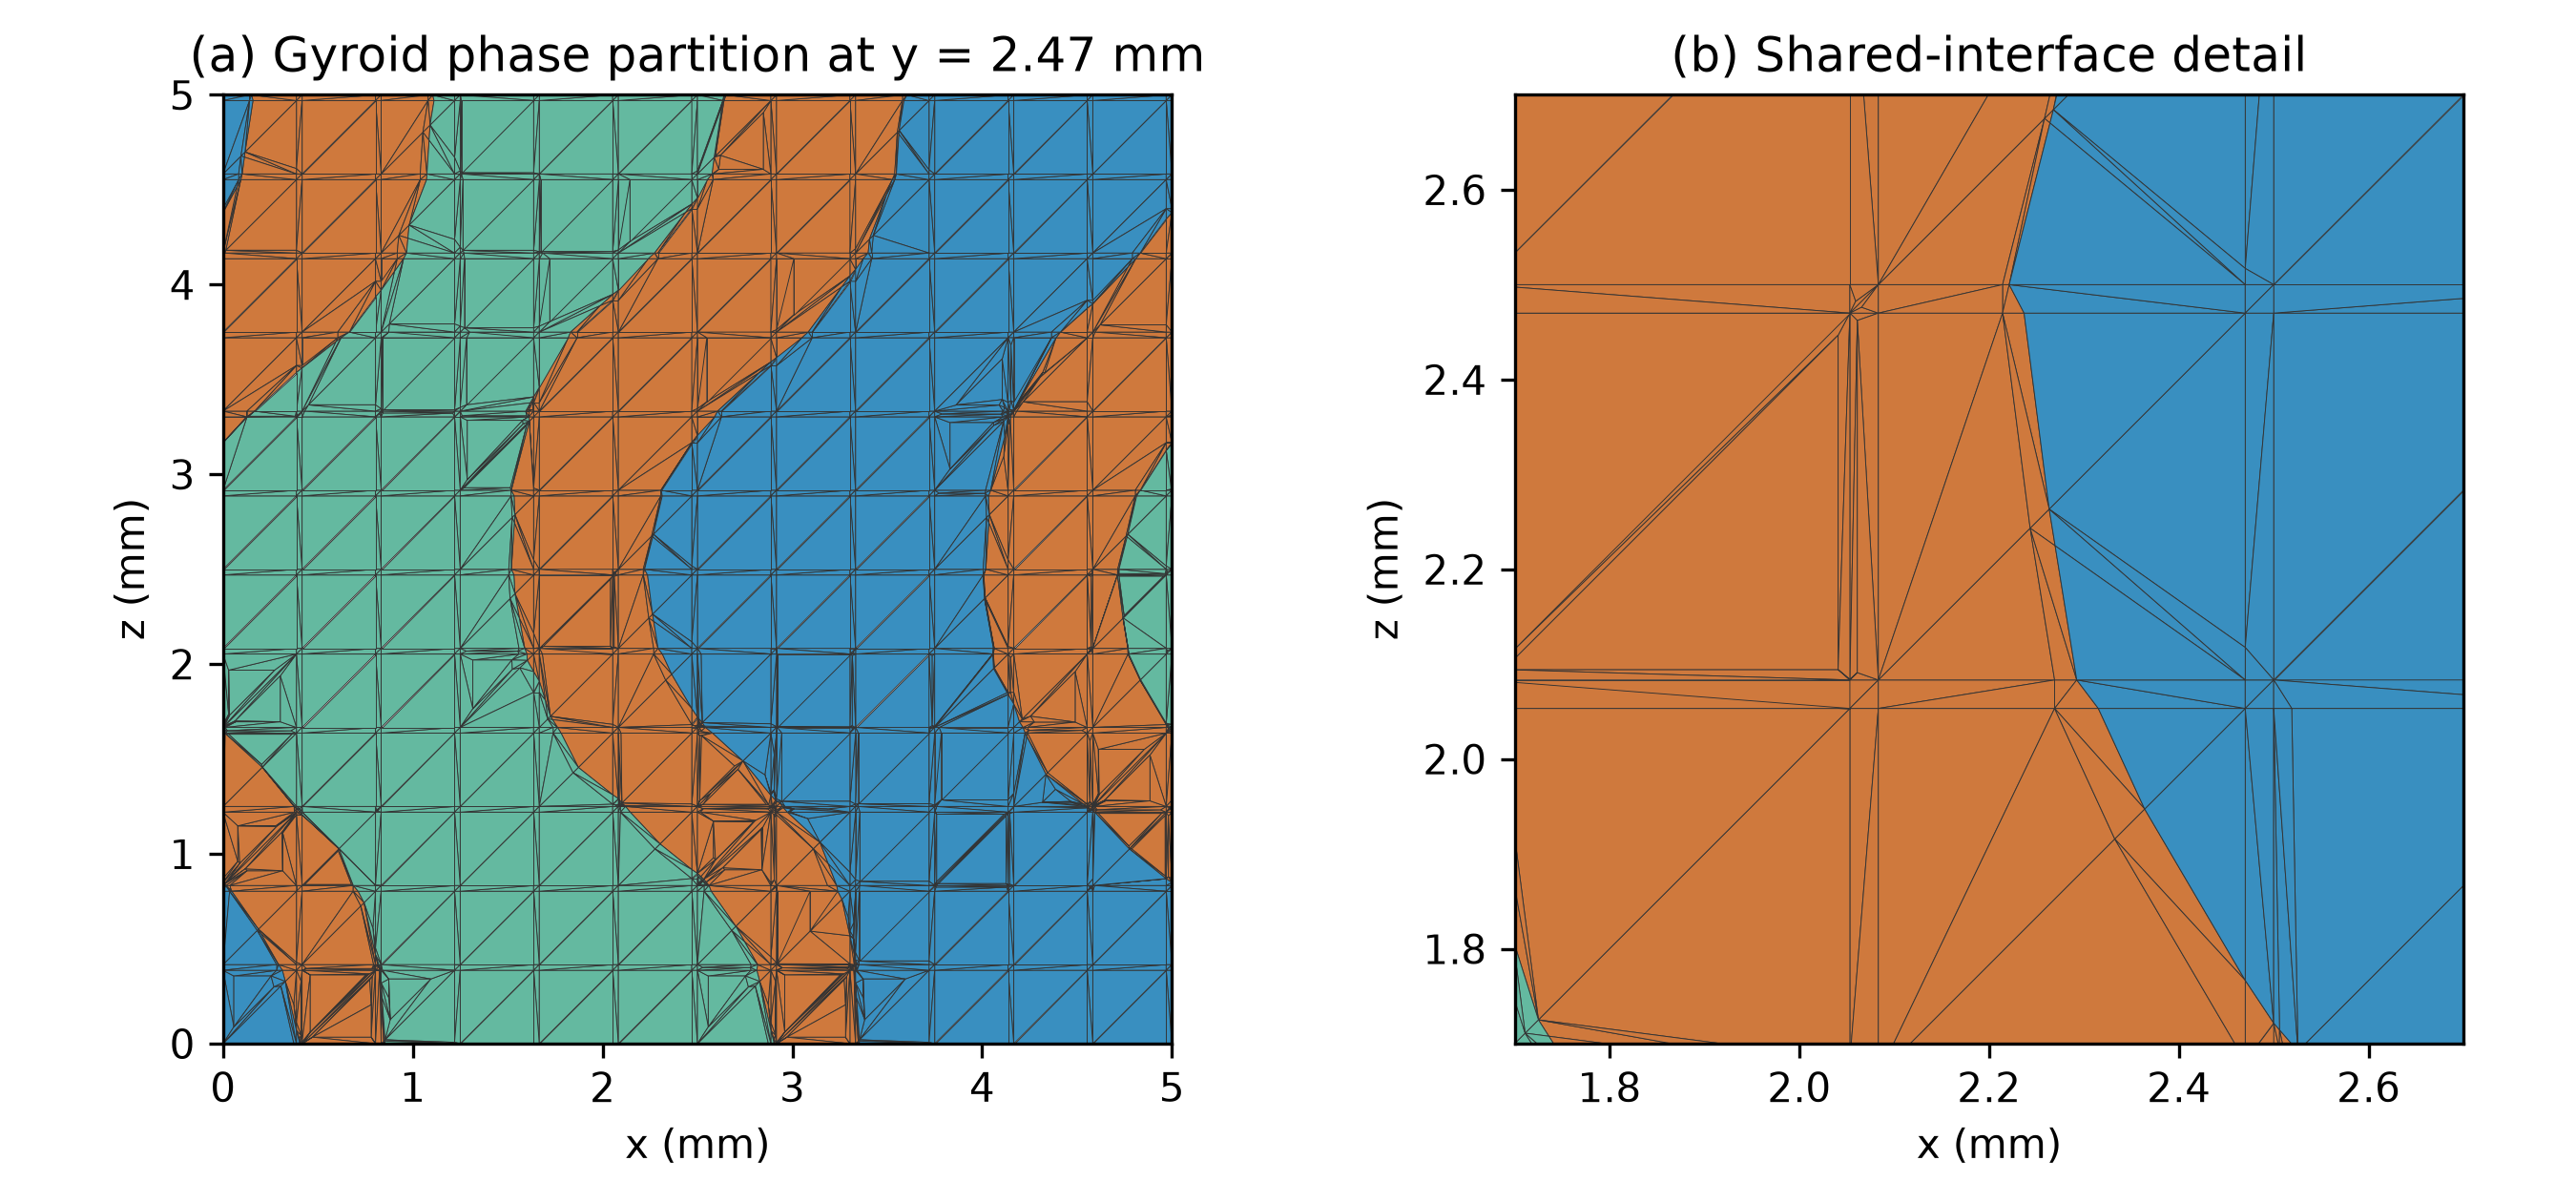
\includegraphics[width=1.0\textwidth]{fig3_interface.png}
\caption{Cross-section through the actual Gyroid tetrahedral mesh at $y=2.47$ mm. Orange identifies solid; blue and green identify the two pore domains. The magnified view shows matching phase-interface intersections. Displayed edges are intersections of tetrahedral faces with the cutting plane.}
\label{fig:interface}
\end{figure}

\begin{minipage}{\textwidth}
\subsection{Sample code snippets}

\begin{lstlisting}[language=Python]
from tpmslab import Config, generate, save_model
from tpmslab.comsol import build_mph

config = Config(
    family="Gyroid", domain_mode="solid_fluid",
    density_start=0.25, density_end=0.50,
    gradient="linear", axis="z", resolution=12,
)
model = generate(config)
folder = save_model(model, "gyroid_solid_fluid")
# Optional licensed COMSOL operation:
build_mph(folder, model["report"], solve=True)
\end{lstlisting}
\end{minipage}

The output directory must be new. For dual-domain models, solve=True invokes the fixed-wall pore-flow demonstration described below. With solve=False, the bridge creates an unsolved mesh-based model with phase materials and named selections for user-defined physics. Solid-only mode remains the default and retains its existing elasticity demonstration.

\FloatBarrier
\section{Illustrative examples}


\begin{figure}[!htbp]
\centering
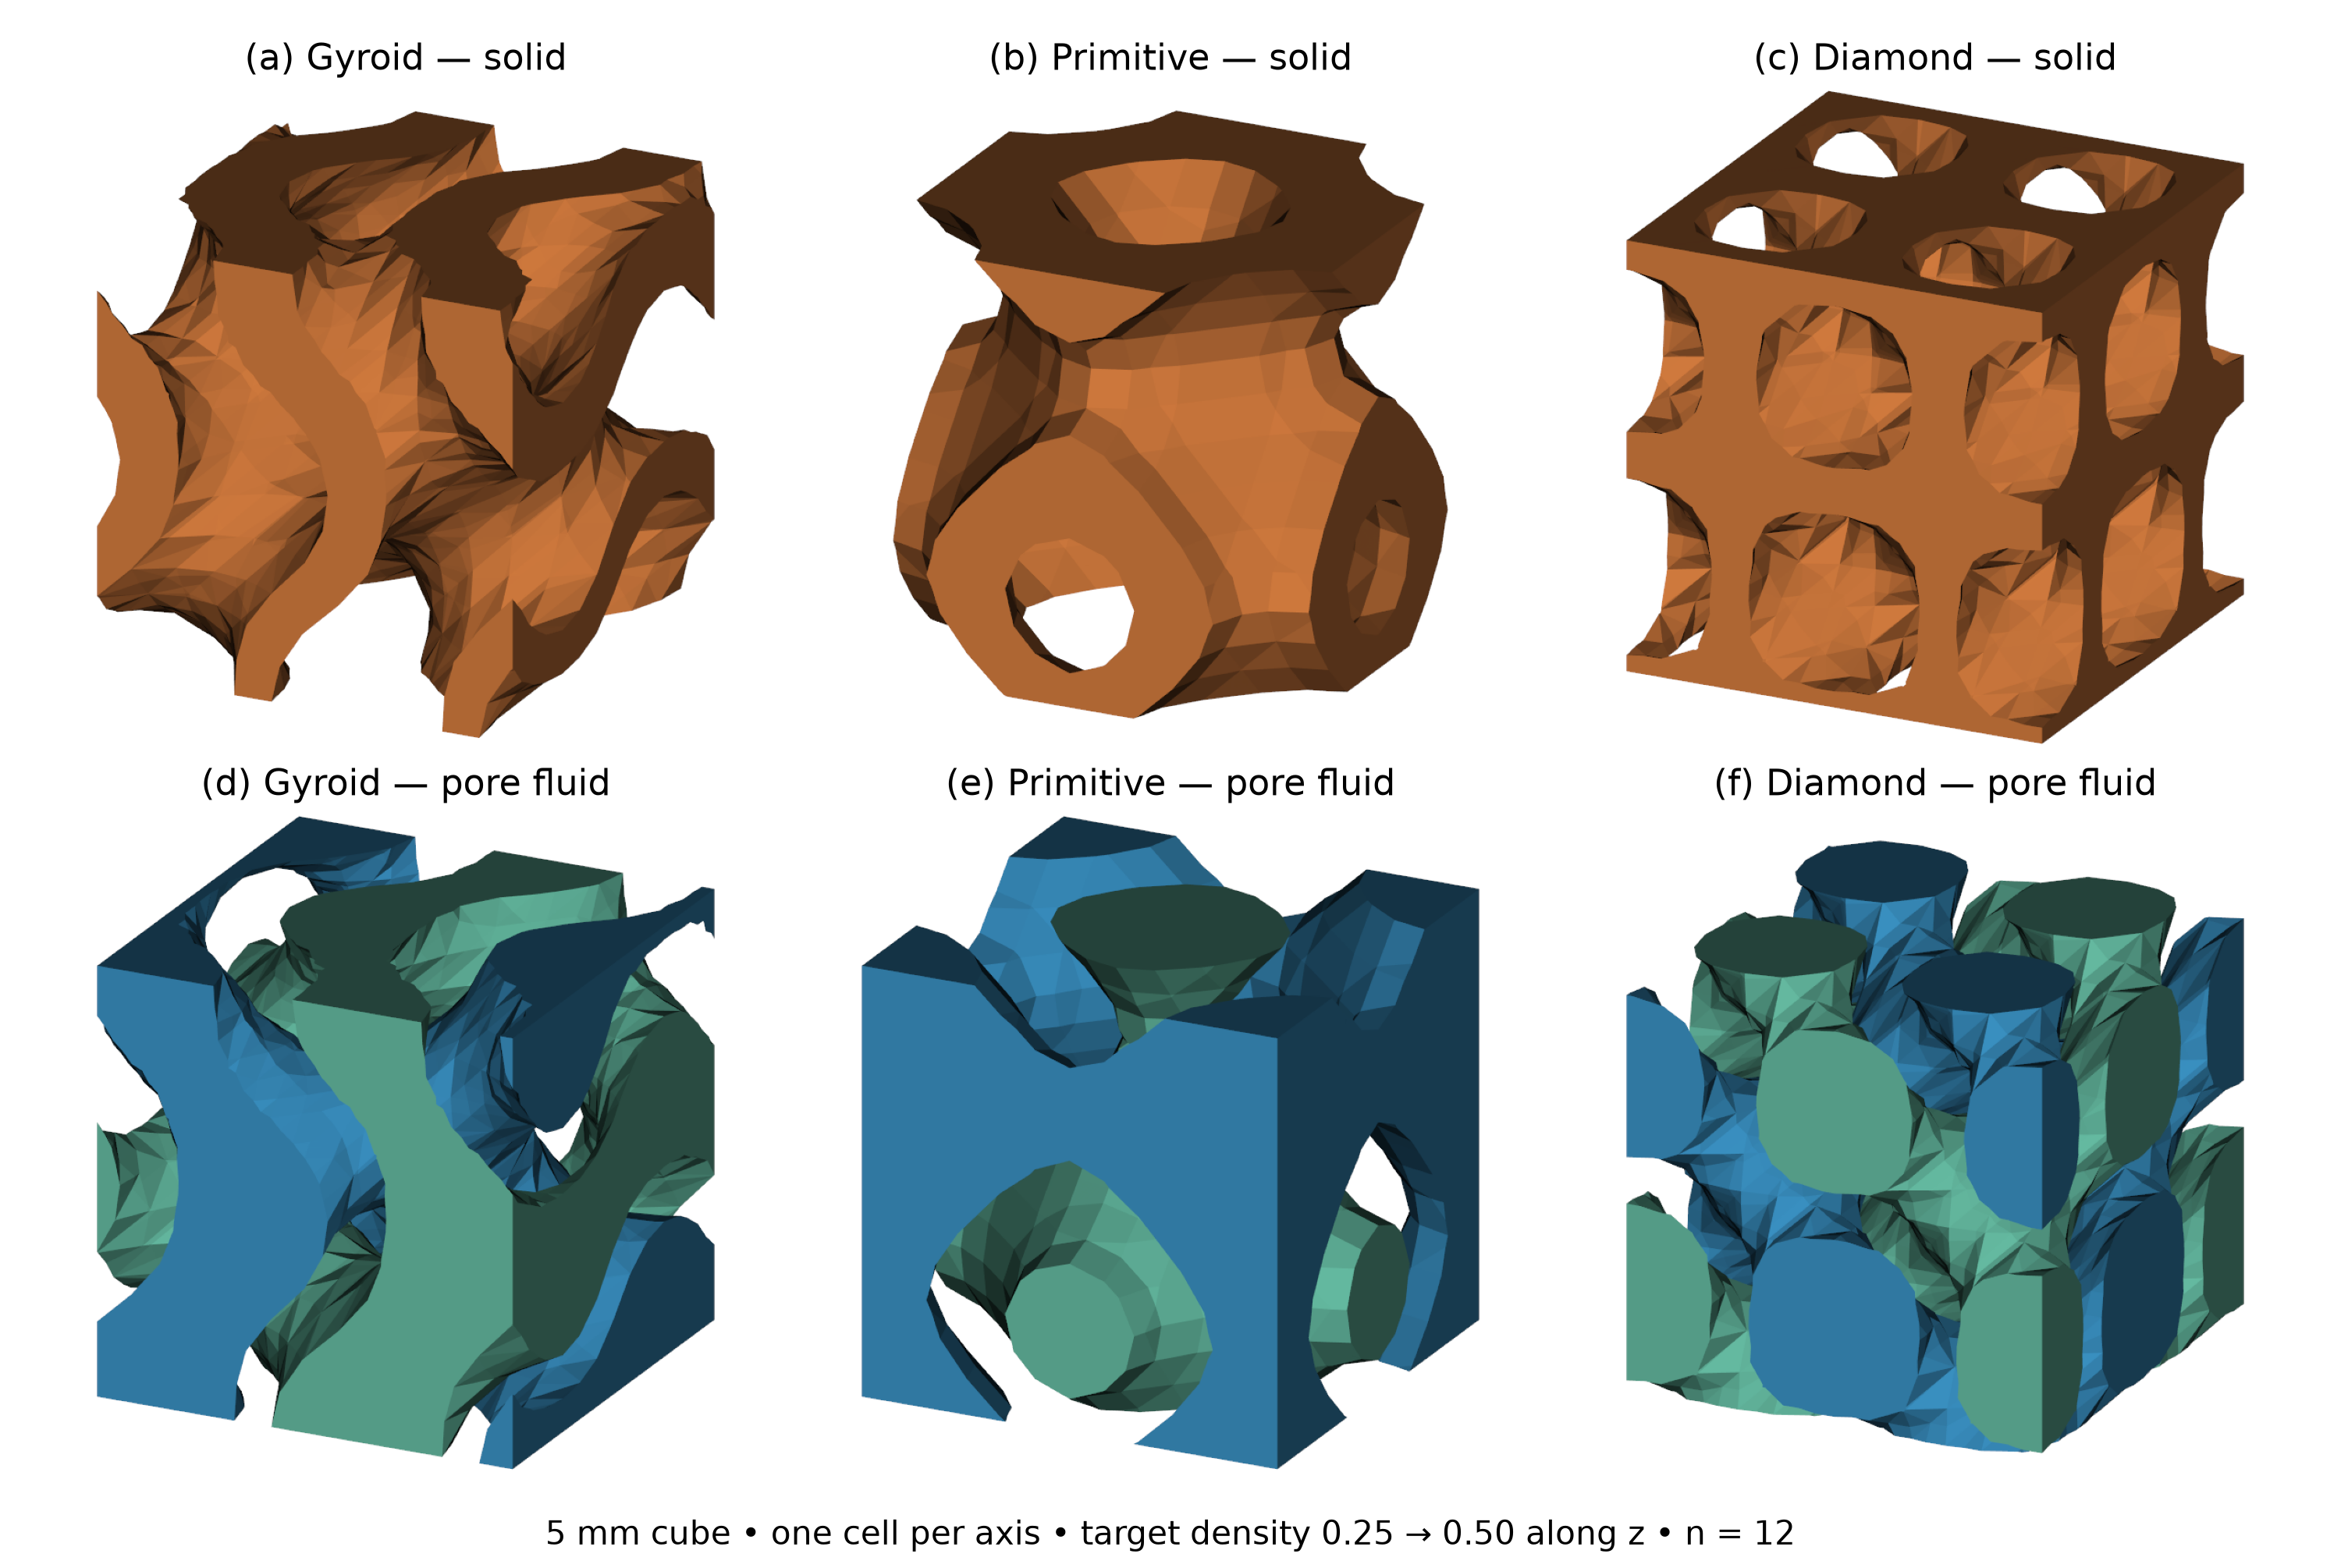
\includegraphics[width=1.0\textwidth]{fig2_geometry.png}
\caption{Actual complementary meshes used in the three pore-flow demonstrations. Orange denotes solid, while blue and green distinguish disconnected fluid domains. All specimens occupy a $5\times5\times5$ mm box; the target density varies linearly from 0.25 to 0.50 along $z$. Faceted surfaces reflect the verified $n=12$ discretization; no surface smoothing is applied.}
\label{fig:geometry}
\end{figure}

\subsection{Automated partition and export checks}

The local test suite contains 77 passing tests. The added tests cover Gyroid, Primitive and Diamond sheets and both network modes. They verify positive element volumes, phase membership, bounding-box volume recovery and exact matching of interface triangle connectivity. An affine-field half-box case supplies an independent geometric reference: in a 5 mm cube, solid and fluid volumes each equal 62.5 mm$^3$ and the planar interface area equals 25 mm$^2$. This case also tests intersections aligned with background vertices and an empty complementary branch of the sheet construction. Archive tests check phase arrays, boundary metadata and NASTRAN properties.

Both triangulation strategies were checked for unchanged combined boundary fingerprints and phase volumes. The browser interface was exercised from an installed wheel, including phase preview switching, dual-domain generation and NASTRAN download. No JavaScript exceptions or horizontal overflow at a 390 px viewport were observed. These checks were executed on Windows with Python 3.12; they are not evidence for every supported platform or dependency version.

\subsection{Solid-only mesh and elasticity checks}

The preceding solid-only release was evaluated using three families, two density profiles and three resolutions, giving 18 paired strategy comparisons. Boundary fingerprints matched in every pair; the maximum paired volume difference was 7.11$\times$10$^{-15}$ mm$^3$. Minimum Q increased by factors of 1.012--4.840 at an element-count cost of 3.56--25.96\%. Median Q decreased in all pairs, and the count below Q=0.01 increased in four pairs. These results quantify a local worst-element trade-off rather than a uniform quality improvement.

Six graded solid-only models were imported, solved, saved and reopened in COMSOL 6.3.0.290. The demonstration used E=1.5 GPa, Poisson ratio 0.3, linear displacement elements, a fixed lower face and a $-$0.005 mm upper-face Z displacement in a 5 mm cube. Paired strain energies differed by 0.16--0.23\%. These are workflow checks; neither triangulation was established as an accurate reference solution.

\subsection{Explicit pore-fluid domains and COMSOL flow calculations}

Figure~\ref{fig:geometry} shows the actual meshes. The new dual-domain examples use the same 5 mm cube, one cell per axis, 12 samples per cell edge, default phases (0$^\circ$, 0$^\circ$, 90$^\circ$), and a linear Z density profile from 0.25 to 0.50. All three geometries contain one connected solid domain and two disconnected pore-fluid domains. Their phase volumes sum to 125 mm$^3$ within numerical precision. Table~\ref{tab:meshes} summarizes mesh sizes and phase volumes.

\begin{table}[!htbp]
\centering\footnotesize
\caption{Complementary solid--fluid meshes at resolution 12. Each specimen contains one solid and two fluid connected domains.}
\label{tab:meshes}
\begin{tabular}{@{}lrrrr@{}}
\toprule
Family & Tetrahedra & \shortstack{Solid volume\\(mm$^3$)} & \shortstack{Fluid volume\\(mm$^3$)} & \shortstack{Interface\\triangles} \\
Gyroid & 38,292 & 49.17571054 & 75.82428946 & 7,392 \\
Primitive Schwartz & 31,282 & 47.92241262 & 77.07758738 & 5,608 \\
Diamond & 42,280 & 50.20485764 & 74.79514236 & 9,072 \\
\bottomrule
\end{tabular}
\end{table}

COMSOL imports were checked for separate solid/fluid selections, individual domain volumes and a nonempty interface selection. The flow demonstration applies the Creeping Flow interface only to fluid domains, using density 1000 kg/m$^3$ and dynamic viscosity 0.001 Pa$\cdot$s. Pressure is 0.01 Pa on the Z$-$ fluid openings and zero on the Z+ openings. The solid--fluid interface and other exterior fluid faces are no-slip walls. Solid deformation is not solved. The automatic demonstration requires every fluid component to reach both Z faces; configurations that fail this condition can still be exported for a custom study.

Figure~\ref{fig:comsol} illustrates actual flow and elasticity solution fields. All three stationary calculations completed and retained their results after saving and reopening. Table~\ref{tab:flow} reports the outlet volume flow and the relative flux imbalance,
\begin{equation}\varepsilon_Q=\frac{|Q_{\mathrm{in}}+Q_{\mathrm{out}}|}{\max(|Q_{\mathrm{in}}|,|Q_{\mathrm{out}}|)},\end{equation}
using outward-signed fluxes. The small imbalance checks consistency of these solutions. It does not establish resolution-independent permeability, near-wall accuracy or general conservation bounds for other configurations.

\begin{table}[!htbp]
\centering\footnotesize
\caption{Actual COMSOL 6.3.0.290 fixed-wall pore-flow results. Imported phase volumes, saved mesh counts and reopened outlet integrals were verified in each case.}
\label{tab:flow}
\begin{tabular}{@{}lrr@{}}
\toprule
Family & Outlet volume flow (m$^3$/s) & Relative flux imbalance \\
Gyroid & 8.89101254$\times$10$^{-10}$ & 1.4318$\times$10$^{-8}$ \\
Primitive Schwartz & 4.45998409$\times$10$^{-10}$ & 1.8174$\times$10$^{-9}$ \\
Diamond & 4.24304079$\times$10$^{-10}$ & 4.6994$\times$10$^{-6}$ \\
\bottomrule
\end{tabular}
\end{table}

The accompanying artifacts contain three unsolved and three solved dual-domain MPH files, mesh arrays, configurations, Java builders, logs and verification records. The benchmark script rebuilds them in a new directory. COMSOL and the required physics licence are external dependencies; the open-source mesh tests do not require them.


\begin{figure}[!htbp]
\centering
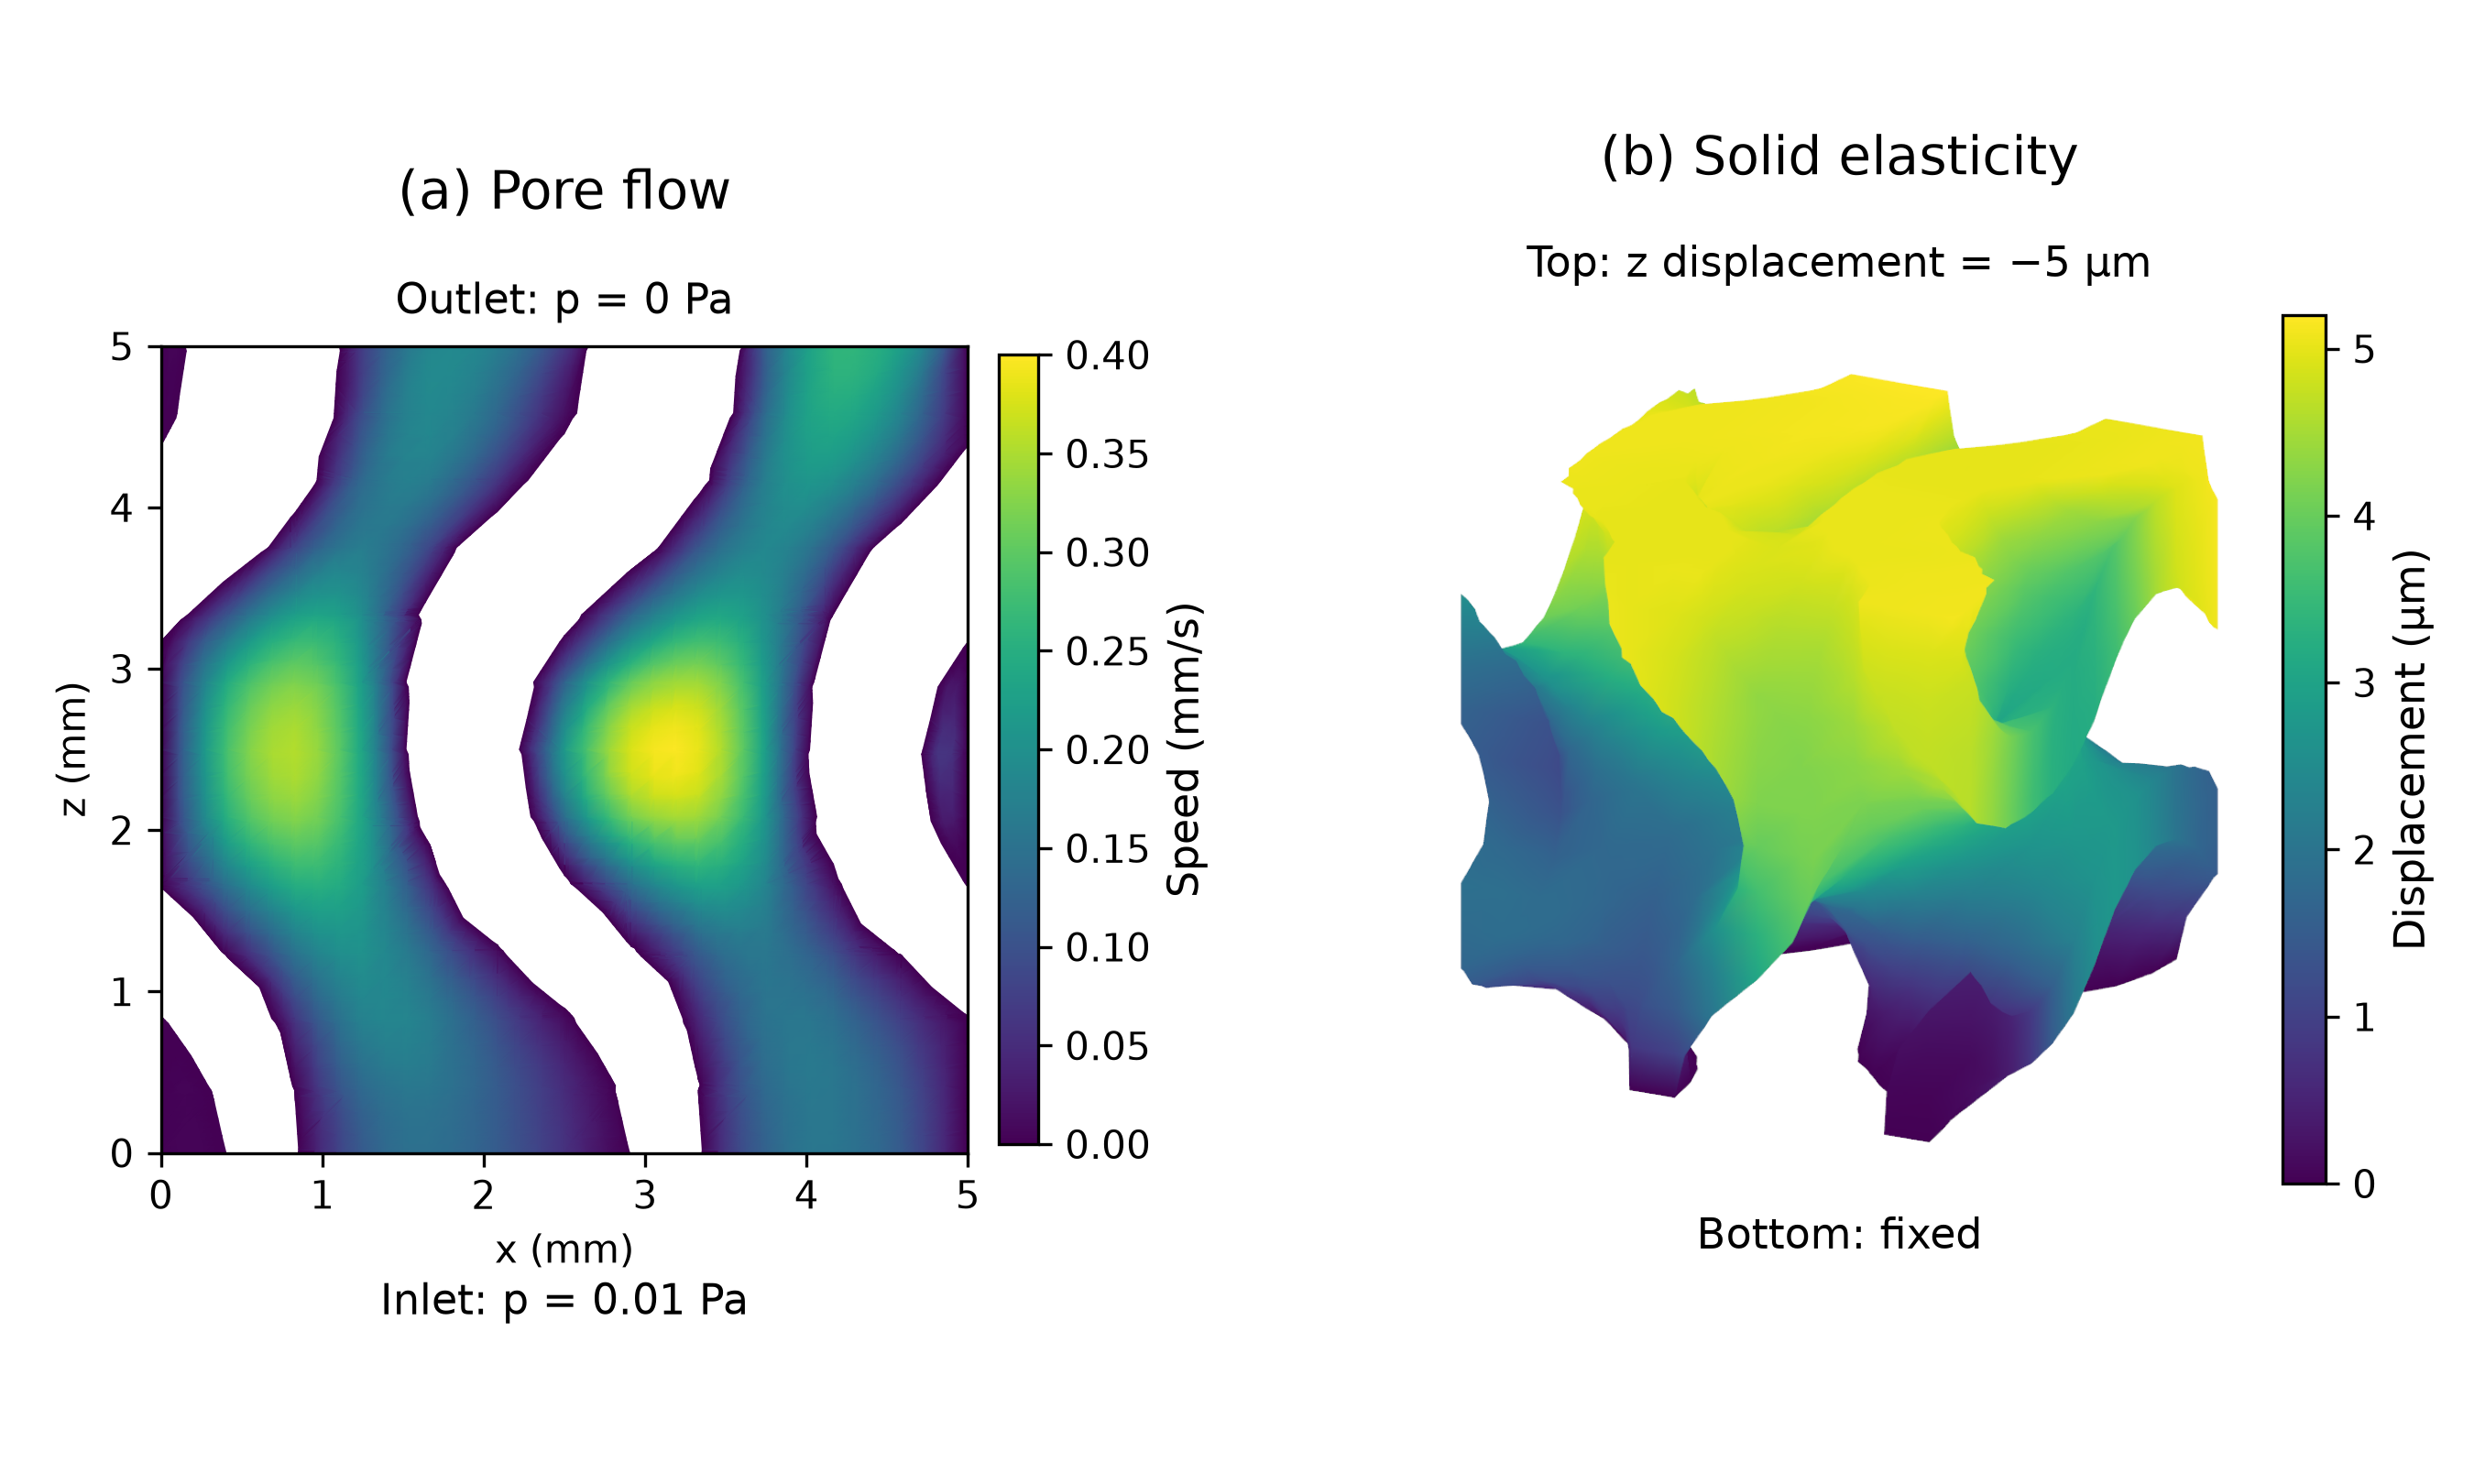
\includegraphics[width=1.0\textwidth]{fig4_comsol.png}
\caption{Results evaluated from saved COMSOL 6.3 solutions for graded Gyroid specimens. (a) Pore-fluid speed on an interior section at $y=2.47$ mm, with a 0.01 Pa pressure drop in $z$ and fixed no-slip walls. (b) Displacement magnitude in the separate solid-only elasticity study: the lower face is fixed and the upper-face $z$ displacement is $-5$ $\mu$m. Geometry is shown undeformed. These are separate calculations, not a coupled fluid--structure simulation. Colors are interpolated from exported finite-element solution values.}
\label{fig:comsol}
\end{figure}

\FloatBarrier
\section{Impact}

The software reduces the number of data transformations required to prepare a graded lattice and its pore space for simulation. A single configuration produces both phases, connected-domain labels and shared interface connectivity. Users can assign solid and fluid materials to named selections rather than reconstructing pore domains manually from a surface preview. The same generator can be used interactively or within Python parameter studies, while reports retain actual phase volumes and mesh-quality diagnostics.

The verified application scope is direct volume-mesh generation, solid-only elasticity workflow checks and fixed-wall pore-flow calculations in COMSOL. The retained interface provides an input for future coupled studies, but this release does not implement or validate deformation-coupled fluid--structure interaction. Conjugate heat transfer, external fluid regions, inlet reservoirs, boundary-layer meshing, contact and geometry-level Boolean operations are also outside the demonstrated scope. No external adoption, time-saving measurement or research publication enabled by this release is claimed.

Current limitations include box-bounded domains, moderate sampling limits, residual small cut elements and approximate density calibration. Rapid gradients and finite specimen boundaries can change measured density relative to the periodic-cell target. Comparisons with independent meshers and solver refinement studies are needed before asserting accuracy or performance advantages. The public release should therefore present the software as an inspectable simulation-preparation tool with explicit verification records.

\FloatBarrier
\section{Conclusions}

TPMS Lab provides a Python workflow for graded TPMS-derived solid and complementary pore-fluid meshes with shared interfaces. Domain-aware exports and a COMSOL bridge preserve phase selections and support actual solver execution. Analytical partition tests, automated regression tests and three saved-and-reopened pore-flow examples establish the reported functionality. Future work should focus on independent meshing comparisons, flow and mechanics convergence, broader geometry support and validated coupled physics.

\section*{CRediT authorship contribution statement}

[Authors must supply named roles reflecting their actual contributions.]

\section*{Declaration of competing interest}

[Authors must confirm and supply an accurate declaration.]

\section*{Funding and acknowledgements}

[Supply actual funding and acknowledgements, or confirm that no specific funding was received.]

\section*{Data and software availability}

The local release contains source, wheel and source distributions, automated tests, reproduction scripts and solver verification artifacts. [Insert permanent public URLs for the exact reviewed code version and validation data before submission. The package has not yet been published on PyPI.]

\section*{Declaration of generative AI and AI-assisted technologies}

OpenAI Codex assisted with software implementation, test preparation and manuscript drafting. [Authors must describe their completed review and take responsibility for the submitted software, analyses and manuscript. This draft does not assert that human review has already occurred.]

\FloatBarrier
\small
\setlength{\bibsep}{3pt}
\bibliographystyle{elsarticle-num}
\bibliography{references}
\end{document}
